% Options for packages loaded elsewhere
\PassOptionsToPackage{unicode}{hyperref}
\PassOptionsToPackage{hyphens}{url}
%
\documentclass[
]{article}
\usepackage{amsmath,amssymb}
\usepackage{lmodern}
\usepackage{ifxetex,ifluatex}
\ifnum 0\ifxetex 1\fi\ifluatex 1\fi=0 % if pdftex
  \usepackage[T1]{fontenc}
  \usepackage[utf8]{inputenc}
  \usepackage{textcomp} % provide euro and other symbols
\else % if luatex or xetex
  \usepackage{unicode-math}
  \defaultfontfeatures{Scale=MatchLowercase}
  \defaultfontfeatures[\rmfamily]{Ligatures=TeX,Scale=1}
\fi
% Use upquote if available, for straight quotes in verbatim environments
\IfFileExists{upquote.sty}{\usepackage{upquote}}{}
\IfFileExists{microtype.sty}{% use microtype if available
  \usepackage[]{microtype}
  \UseMicrotypeSet[protrusion]{basicmath} % disable protrusion for tt fonts
}{}
\makeatletter
\@ifundefined{KOMAClassName}{% if non-KOMA class
  \IfFileExists{parskip.sty}{%
    \usepackage{parskip}
  }{% else
    \setlength{\parindent}{0pt}
    \setlength{\parskip}{6pt plus 2pt minus 1pt}}
}{% if KOMA class
  \KOMAoptions{parskip=half}}
\makeatother
\usepackage{xcolor}
\IfFileExists{xurl.sty}{\usepackage{xurl}}{} % add URL line breaks if available
\IfFileExists{bookmark.sty}{\usepackage{bookmark}}{\usepackage{hyperref}}
\hypersetup{
  pdftitle={README.Rmd},
  hidelinks,
  pdfcreator={LaTeX via pandoc}}
\urlstyle{same} % disable monospaced font for URLs
\usepackage[margin=1in]{geometry}
\usepackage{color}
\usepackage{fancyvrb}
\newcommand{\VerbBar}{|}
\newcommand{\VERB}{\Verb[commandchars=\\\{\}]}
\DefineVerbatimEnvironment{Highlighting}{Verbatim}{commandchars=\\\{\}}
% Add ',fontsize=\small' for more characters per line
\usepackage{framed}
\definecolor{shadecolor}{RGB}{248,248,248}
\newenvironment{Shaded}{\begin{snugshade}}{\end{snugshade}}
\newcommand{\AlertTok}[1]{\textcolor[rgb]{0.94,0.16,0.16}{#1}}
\newcommand{\AnnotationTok}[1]{\textcolor[rgb]{0.56,0.35,0.01}{\textbf{\textit{#1}}}}
\newcommand{\AttributeTok}[1]{\textcolor[rgb]{0.77,0.63,0.00}{#1}}
\newcommand{\BaseNTok}[1]{\textcolor[rgb]{0.00,0.00,0.81}{#1}}
\newcommand{\BuiltInTok}[1]{#1}
\newcommand{\CharTok}[1]{\textcolor[rgb]{0.31,0.60,0.02}{#1}}
\newcommand{\CommentTok}[1]{\textcolor[rgb]{0.56,0.35,0.01}{\textit{#1}}}
\newcommand{\CommentVarTok}[1]{\textcolor[rgb]{0.56,0.35,0.01}{\textbf{\textit{#1}}}}
\newcommand{\ConstantTok}[1]{\textcolor[rgb]{0.00,0.00,0.00}{#1}}
\newcommand{\ControlFlowTok}[1]{\textcolor[rgb]{0.13,0.29,0.53}{\textbf{#1}}}
\newcommand{\DataTypeTok}[1]{\textcolor[rgb]{0.13,0.29,0.53}{#1}}
\newcommand{\DecValTok}[1]{\textcolor[rgb]{0.00,0.00,0.81}{#1}}
\newcommand{\DocumentationTok}[1]{\textcolor[rgb]{0.56,0.35,0.01}{\textbf{\textit{#1}}}}
\newcommand{\ErrorTok}[1]{\textcolor[rgb]{0.64,0.00,0.00}{\textbf{#1}}}
\newcommand{\ExtensionTok}[1]{#1}
\newcommand{\FloatTok}[1]{\textcolor[rgb]{0.00,0.00,0.81}{#1}}
\newcommand{\FunctionTok}[1]{\textcolor[rgb]{0.00,0.00,0.00}{#1}}
\newcommand{\ImportTok}[1]{#1}
\newcommand{\InformationTok}[1]{\textcolor[rgb]{0.56,0.35,0.01}{\textbf{\textit{#1}}}}
\newcommand{\KeywordTok}[1]{\textcolor[rgb]{0.13,0.29,0.53}{\textbf{#1}}}
\newcommand{\NormalTok}[1]{#1}
\newcommand{\OperatorTok}[1]{\textcolor[rgb]{0.81,0.36,0.00}{\textbf{#1}}}
\newcommand{\OtherTok}[1]{\textcolor[rgb]{0.56,0.35,0.01}{#1}}
\newcommand{\PreprocessorTok}[1]{\textcolor[rgb]{0.56,0.35,0.01}{\textit{#1}}}
\newcommand{\RegionMarkerTok}[1]{#1}
\newcommand{\SpecialCharTok}[1]{\textcolor[rgb]{0.00,0.00,0.00}{#1}}
\newcommand{\SpecialStringTok}[1]{\textcolor[rgb]{0.31,0.60,0.02}{#1}}
\newcommand{\StringTok}[1]{\textcolor[rgb]{0.31,0.60,0.02}{#1}}
\newcommand{\VariableTok}[1]{\textcolor[rgb]{0.00,0.00,0.00}{#1}}
\newcommand{\VerbatimStringTok}[1]{\textcolor[rgb]{0.31,0.60,0.02}{#1}}
\newcommand{\WarningTok}[1]{\textcolor[rgb]{0.56,0.35,0.01}{\textbf{\textit{#1}}}}
\usepackage{graphicx}
\makeatletter
\def\maxwidth{\ifdim\Gin@nat@width>\linewidth\linewidth\else\Gin@nat@width\fi}
\def\maxheight{\ifdim\Gin@nat@height>\textheight\textheight\else\Gin@nat@height\fi}
\makeatother
% Scale images if necessary, so that they will not overflow the page
% margins by default, and it is still possible to overwrite the defaults
% using explicit options in \includegraphics[width, height, ...]{}
\setkeys{Gin}{width=\maxwidth,height=\maxheight,keepaspectratio}
% Set default figure placement to htbp
\makeatletter
\def\fps@figure{htbp}
\makeatother
\setlength{\emergencystretch}{3em} % prevent overfull lines
\providecommand{\tightlist}{%
  \setlength{\itemsep}{0pt}\setlength{\parskip}{0pt}}
\setcounter{secnumdepth}{-\maxdimen} % remove section numbering
\ifluatex
  \usepackage{selnolig}  % disable illegal ligatures
\fi

\title{README.Rmd}
\author{}
\date{\vspace{-2.5em}}

\begin{document}
\maketitle

\hypertarget{introduction}{%
\section{Introduction}\label{introduction}}

The goal of this package is to segment events in a CNV's profile based
on the \(log_2\) ratio and the genomic position using a regression tree
approach. A \(log_2\) ratio above zero means that there is a
amplification in copy number in the sample genome compared to the
reference genome. On the other hand, if the \(log_2\) ratio is below
zero then there is a deletion in the copy number in the sample genome
compared to the reference genome.

This package provides a way to segment a CNV's profile and visualize the
segmentation of individual chromosomes and the full genome.

\hypertarget{installation}{%
\subsection{Installation}\label{installation}}

To install the most updated version of this package use the following:

\begin{Shaded}
\begin{Highlighting}[]
\FunctionTok{install.packages}\NormalTok{(}\StringTok{"devtools"}\NormalTok{)}
\FunctionTok{library}\NormalTok{(devtools)}
\NormalTok{devtools}\SpecialCharTok{::}\FunctionTok{install\_github}\NormalTok{(}\StringTok{"annikacleven/regtreeseg"}\NormalTok{)}
\end{Highlighting}
\end{Shaded}

\hypertarget{resources}{%
\subsection{Resources}\label{resources}}

The regtreeseg vignette includes sample code on how to use each of the
segmenting functions. The vignette also dives into optional operations
of the functions and more details on the complexity parameter used to
segment the genomic data. The vignette is available upon download of the
package.

\hypertarget{overview}{%
\subsection{Overview}\label{overview}}

Using a regression tree approach set up in the `rpart' package, CNV
\(log_2\) ratio data can be segmented with multiple approaches. In the
regression tree approaches the response variable is the \(log_2\) ratio
and the explanatory variable is the genomic location. Therefore the data
is partitioned into segments that predict the \(log_2\) ratio for the
genomic positions in each segment. In regtreeseg, the regression trees
use the complexity parameter optimized to have the minimum cross
validation error. The complexity parameter is the minimum increase in
the \(R^2\) that the split in the regression tree must create for the
split to be included. The innovation of this package is using an
iteration of regression trees to create a regression tree that catches
all events in the CNV profile. Beyond the iteration, an option to weight
points farther from the \(log_2\) ratio of 0 is available.

There are three segmentation methods in this package:

\begin{enumerate}
\def\labelenumi{\arabic{enumi}.}
\item
  Segmentation using an optimal complexity parameter (cp)
\item
  Segmentation using an optimal cp value and 3 regression tree
  iterations
\item
  Segmentation using an optimal cp value, 3 regression tree iterations,
  and weighting
\end{enumerate}

Each of the segmentation methods in this package follow a general path.

\begin{center}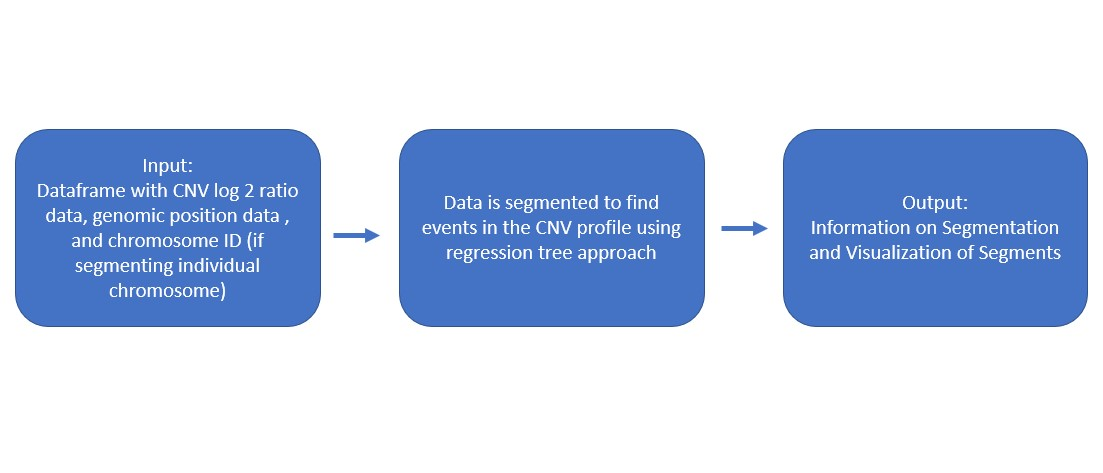
\includegraphics[width=1\linewidth]{/home/mayo/m252318/R/functionworkflow2.png} \end{center}

The use of an iterative regression tree approach allows for the tree to
catch events in the CNV profile on the first round and then catch other
less prominent events in the next iterations. This approach identifies
more CNV events, than a single regression tree.

To begin the iterative regression tree approach, the data is segmented
using a regression tree with the optimal complexity parameter (unless
specified otherwise). The predictions from this regression tree are the
first iteration (pred1). Then the residual error is calculated. Using
the optimal complexity parameter (cp) for this residual data a
regression tree is fitted to the data. This regression tree predicts the
spikes in the residual error with an explanatory variable of the genomic
location (pred2). Then the predictions from the initial regression tree
(pred1) and the second regression tree (pred2) are added together to
create a new prediction. Then a third iteration follows. The residuals
are calculated from the combined prediction of pred1+pred2 and using the
cpopt another regression tree is fitted to this residual data (pred3).
Then the predictions from each iteration are added together
(pred1+pred2+pred3) for the final prediction.

\begin{center}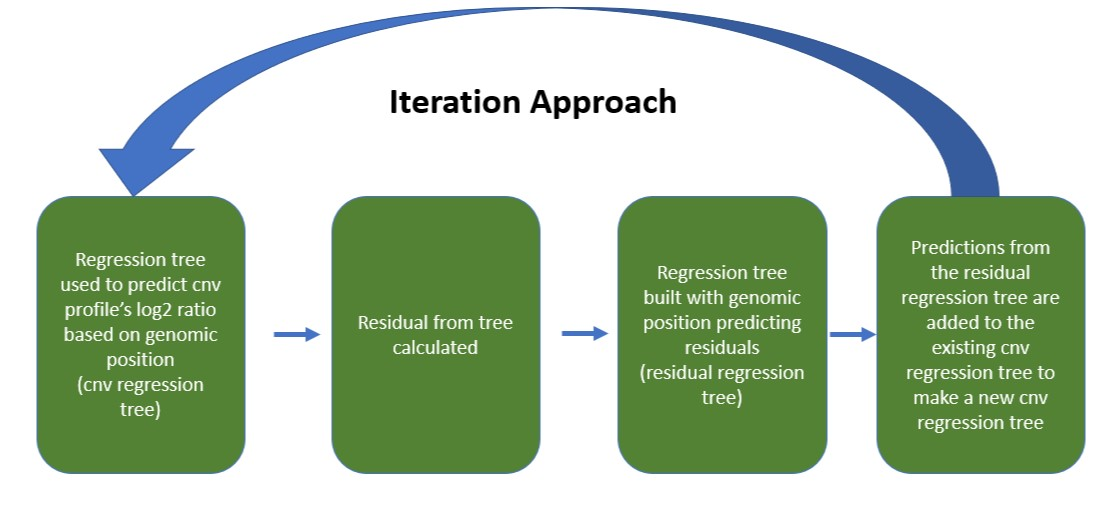
\includegraphics[width=1\linewidth]{/home/mayo/m252318/R/iteration} \end{center}

The functions in this package segment either a single chromosome or the
full genome. When segmenting the full genome each chromosome is
segmented separately and then each chromosome's segmentation is included
in a full report.

\hypertarget{demonstration}{%
\subsection{Demonstration}\label{demonstration}}

More detailed instructions on how to execute each of the segmentation
methods can be viewed in the vignette. Here a description of the flow of
the function and an example of how to use the iterative regression tree
approach with optimal cp values for a single chromosome is provided.

\begin{center}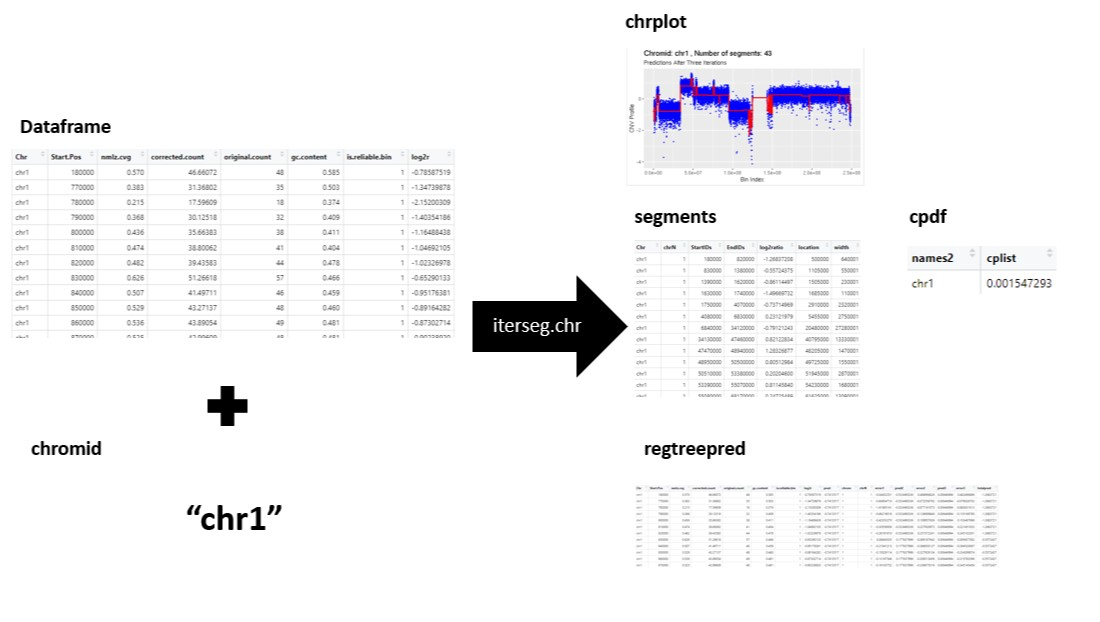
\includegraphics[width=1\linewidth]{/home/mayo/m252318/R/itersegworkflow} \end{center}

\begin{Shaded}
\begin{Highlighting}[]
\FunctionTok{library}\NormalTok{(regtreeseg)}
\FunctionTok{data}\NormalTok{(}\StringTok{"chr3sample"}\NormalTok{)}
\NormalTok{demo }\OtherTok{\textless{}{-}} \FunctionTok{iterseg.chr}\NormalTok{(chr3sample, }\AttributeTok{chromid =} \StringTok{"chr3"}\NormalTok{)}
\NormalTok{demo}\SpecialCharTok{$}\NormalTok{chrplot}
\NormalTok{demo}\SpecialCharTok{$}\NormalTok{segments}
\end{Highlighting}
\end{Shaded}

A screenshot of the chrplot is shown below:

\begin{center}\includegraphics[width=1\linewidth]{/home/mayo/m252318/R/iterchrchr3sample} \end{center}

\hypertarget{dataframe-input-specification}{%
\subsection{Dataframe input
specification}\label{dataframe-input-specification}}

The inputs of these functions require a dataframe that has column names
specifically labeled as ``Start.Pos'', ``log2r'', and ``Chr''. The
``Start.Pos'' column is the bin index or genomic location which the
log2ratio comes from. The ``log2r'' column is the log2ratio that between
the sample genome ad the reference genome. The ``Chr'' column is the
chromosome of interest. The chromosomes should be labeled exactly as
``chr1'', ``chr2'', ``chr22'', ``chrX'', ``chrY''.

\end{document}
